\usepackage{xcolor}
\definecolor{orbitCyan}{HTML}{137DA0}
\definecolor{orbitViolet}{HTML}{6D4AA6}
\definecolor{orbitAmber}{HTML}{AC6A15}
\AtBeginDocument{\hypersetup{colorlinks=true,urlcolor=orbitCyan,linkcolor=orbitViolet}}
\AtBeginDocument{\renewcommand{\contentsname}{Table des matières}}
\renewcommand{\maketitle}{\begin{titlepage}\centering
\vspace*{0.7in}
{\color{orbitAmber}\Huge\bfseries Orbit}\par\vspace{0.25in}
{\LARGE Jouer, comprendre, transmettre}\par\vspace{0.2in}
{\large Les quinze interactions de l’atome, du geste au code}\par\vspace{0.55in}
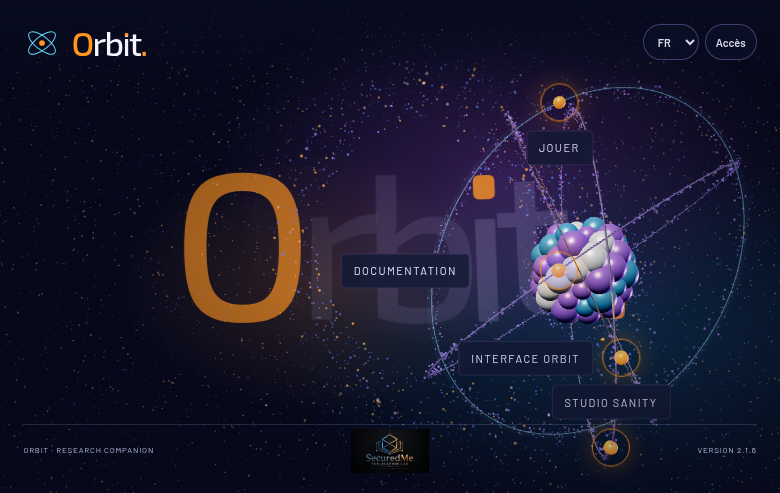
\includegraphics[width=\textwidth]{figures/landing-final.png}\par\vspace{0.55in}
{\color{orbitViolet}\rule{0.65\textwidth}{0.8pt}}\par\vspace{0.2in}
{\large Jean-Sébastien Beaulieu}\par\vspace{0.1in}
Support pédagogique préparé avec Codex\par\vfill
30 septembre 2026 · version 2.1.6\par
\end{titlepage}}
\usepackage{fvextra}
\DefineVerbatimEnvironment{Highlighting}{Verbatim}{commandchars=\\\{\},breaklines,breakanywhere,fontsize=\footnotesize}
\setlength{\emergencystretch}{3em}
\usepackage{fancyhdr}
\pagestyle{fancy}
\fancyhf{}
\fancyhead[L]{\small Orbit · comprendre et transmettre}
\fancyfoot[R]{\thepage}
\renewcommand{\headrulewidth}{0.3pt}
